\documentclass{beamer}
\usepackage{inconsolata}
\usepackage{color}
\usepackage{listings}
\usepackage{cooltooltips}
\usepackage{hyperref}
\usepackage[normalem]{ulem}
\setbeamertemplate{navigation symbols}{}%remove navigation symbols
\usepackage{listings}
\usepackage{color}
\usepackage{framed}

\definecolor{background}{RGB}{39, 40, 34}
\definecolor{string}{RGB}{230, 219, 116}
\definecolor{comment}{RGB}{117, 113, 94}
\definecolor{normal}{RGB}{248, 248, 242}
\definecolor{identifier}{RGB}{166, 226, 46}



\lstset{
  language=C,               			% choose the language of the code
  alsolanguage=Python,            			% choose the language of the code
  alsolanguage=Java,            			% choose the language of the code
  numbers=none,                   		% where to put the line-numbers
  stepnumber=1,                   		% the step between two line-numbers.        
  numbersep=5pt,                  		% how far the line-numbers are from the code
  extendedchars=true,
  numberstyle=\tiny\color{black}\ttfamily,
  backgroundcolor=\color{background},  		% choose the background color. You must add \usepackage{color}
  showspaces=false,               		% show spaces adding particular underscores
  showstringspaces=false,         		% underline spaces within strings
  showtabs=false,                 		% show tabs within strings adding particular underscores
  frame=single,
  framerule=0pt,
  tabsize=4,                      		% sets default tabsize to 2 spaces
  captionpos=n,                   		% sets the caption-position to bottom
  breaklines=true,                		% sets automatic line breaking
  breakatwhitespace=true,         		% sets if automatic breaks should only happen at whitespace
  title=\lstname,                 		% show the filename of files included with \lstinputlisting;
  basicstyle=\color{normal}\tiny\ttfamily,					% sets font style for the code
  keywordstyle=\color{magenta}\tiny\ttfamily,	% sets color for keywords
  stringstyle=\color{string}\tiny\ttfamily,		% sets color for strings
  commentstyle=\color{comment}\tiny\ttfamily,	% sets color for comments
  emph={True, False, format_string, eff_ana_bf, permute, eff_ana_btr, KeyError,
  ValueError, ZeroDivisionError},
  emphstyle=\color{identifier}\tiny\ttfamily,
  morekeywords={with, as}
}

\lstset{literate=%
   *{0}{{{\color{cyan}0}}}1
    {1}{{{\color{cyan}1}}}1
    {2}{{{\color{cyan}2}}}1
    {3}{{{\color{cyan}3}}}1
    {4}{{{\color{cyan}4}}}1
    {5}{{{\color{cyan}5}}}1
    {6}{{{\color{cyan}6}}}1
    {7}{{{\color{cyan}7}}}1
    {8}{{{\color{cyan}8}}}1
    {9}{{{\color{cyan}9}}}1
}



\hypersetup{
  colorlinks=true,
  urlcolor=pink,
}

\title{Python 101}
\subtitle{Lec03 \\ Functions}
\author{thoum}

\begin{document}
\frame{\titlepage}

\begin{frame}
\frametitle{Functions}
  $$f(x) = x+1$$
  $$f(x) = \ln x$$
  %Fibonacci.
  %$$f(x) = f(x-1) + f(x-2)$$
\end{frame}

\begin{frame}[fragile]
\frametitle{Python Functions}
\begin{lstlisting}
def f(x):
    # code block belonging to the function
    r = x+1
    return r
# end of function

def g(x):
    return math.log(x)

# Note that each x is unique to the function

# Calling the function
print(f(3)) # f(3) == 4
print(f(3))
\end{lstlisting}
\end{frame}
\begin{frame}
\frametitle{Why Functions?}
  \begin{itemize}
    \item Reusability
    \item Abstraction
    \item And many more
  \end{itemize}
\end{frame}

\begin{frame}
\frametitle{Reusability}
  \begin{lstinputlisting}
    {./not_reuse.py}
  \end{lstinputlisting}
\end{frame}

\begin{frame}
\frametitle{Reusability}
  \begin{lstinputlisting}
    {./reusability.py}
  \end{lstinputlisting}
\end{frame}

\begin{frame}
\frametitle{Reusability}
\begin{itemize}
  \item Less code to read
  \item Fix once, fix everywhere
  \item DRY: Don't Repeat Yourself
\end{itemize}
\end{frame}

\begin{frame}[fragile]{Abstraction}
  \begin{lstlisting}
print()
  \end{lstlisting}
  vs
  \begin{lstinputlisting}
    {./print_code.c}
  \end{lstinputlisting}
\end{frame}

\begin{frame}{Abstraction}
  \begin{itemize}
    \item Lets us focus
  \end{itemize}
\end{frame}

\begin{frame}{Understanding Functions: Pure}
  \begin{lstinputlisting}
    {./pure_function.py}
  \end{lstinputlisting}
\end{frame}

\begin{frame}{Understanding Functions: Impure}
  \begin{lstinputlisting}
    {./side_effect.py}
  \end{lstinputlisting}
\end{frame}

\begin{frame}{Understanding Functions: Impure}
  \begin{lstinputlisting}
    {./side_effect2.py}
  \end{lstinputlisting}
\end{frame}

\begin{frame}{Detour: Understanding Binding}
  Function parameters and variables can be thought as labels.\\

  The variables names(labels) are \textit{local} to the function,
  called the $scope$ of the variable.
\end{frame}

\begin{frame}[fragile]{Detour: Understanding Binding}
  Here, the local $l$ points to the same list $x$ is pointing.

  By $l[0]=3$, that list(the one $x,y$ is pointing)'s first element points to 3.

  Thus, it changes x.
  \begin{lstlisting}
x = [1,2,3]
def change_element_of_list(l):
    l[0] = 3
change_element_of_list(x)
print(x)
  \end{lstlisting}
\end{frame}

\begin{frame}[fragile]{Detour: Understanding Binding}
  Here, the local $y$ points to the same 3 $x$ is pointing.

  By $y = 4$, the local $y$ now points to 4.
  ($x, y$ nows points to different things)

  Thus, $x==3$.
  \begin{lstlisting}
x = 3
def change_4(y):
    print(y)
    y = 4
    print(y)
change_4(x)
print('x is now:', x)
  \end{lstlisting}
\end{frame}

\begin{frame}[fragile]{Detour: Understanding Binding}
  We use $global$ to $assign$ value to a name defined outside the function.
  We can use the values without using $global$, but not recommended in large
  programs as it is unclear where the variable was defined.
  \begin{lstlisting}
y = [1,2,3]
def change_by_global():
    global y
    y = 3
print(y)
  \end{lstlisting}
\end{frame}

\begin{frame}[fragile]{Detour: Understanding Binding}
  Here, the global $y$ points to the $y$ outside the function.

  By $y = 4$, the global $y$ now points to 4.

  Thus, $y$ is changed.
  \begin{lstlisting}
y = [1,2,3]
def change_by_global():
    global y
    y = 3
print(y)
  \end{lstlisting}
\end{frame}

\begin{frame}{Detour: Understanding Binding}
  \href{https://stackoverflow.com/questions/575196/why-can-a-function-modify-some-arguments-as-perceived-by-the-caller-but-not-oth}{Click
  for details.}
\end{frame}

\begin{frame}[fragile]{Function Practice}
  Choose any code we have written (giving grades? printing stars? is
  string a palindrome?) and turn it to a function.

  \begin{lstlisting}
def stars(n):
    for i in range(1, n+1):
        print('*' * i)

stars(int(input()))
  \end{lstlisting}
\end{frame}

\begin{frame}{Recursion}
  What is recursion?  It is...
\end{frame}

\begin{frame}{Recursion}
  What is recursion?  It is...
\end{frame}

\begin{frame}{Recursion}
  
\includegraphics[width=100mm]{./recursion.png}
\end{frame}

\begin{frame}{Recursion}
  A thing is defined in terms of itself or of its type.
\end{frame}

\begin{frame}{Back to highschool}
  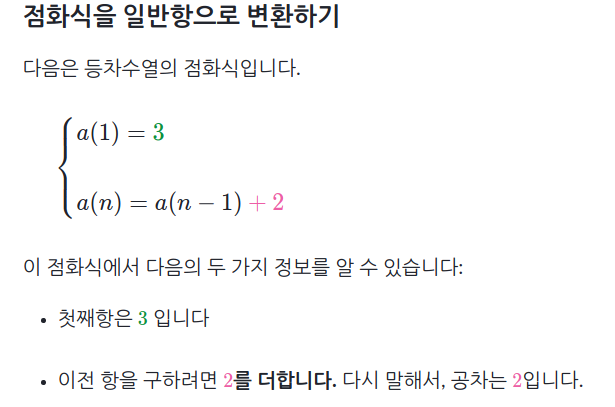
\includegraphics[width=100mm]{./jumhwasik.png}\\
  *\tiny{https://ko.khanacademy.org/}
  
\end{frame}

\begin{frame}[fragile]{In Python}
  \begin{lstinputlisting}
    {./jumhwa.py}
  \end{lstinputlisting}
\end{frame}

\begin{frame}{In English}
  Assume $a(x)$ will somehow, magically calculate $a(n)$\\
  Then, write out the definition, we are done.
\end{frame}

\begin{frame}{How it works}
  Calling $a(3)$.
  \begin{align*}
a(3) = &a(2) + 2\\
&a(2) = a(1) + 2\\
    &\phantom{{ab}={ab}} a(1) = 3\\
    &a(2) = 5\\
a(3) = &7
  \end{align*}
  What if $a(1)$ is not defined?\\
\end{frame}

\begin{frame}{Importance of Base Case}
  $a(-1) \rightarrow a(-2) \rightarrow a(-3) ...$


  \textcolor{red}{Forever and ever}
  until we run out of memory.\footnote{Or not, look up
  \href{https://www.google.com/search?q=call+stack}{call stack} and
  \href{https://www.google.com/search?q=tail+call+optimization}{tail call
  optimization}}
\end{frame}

\begin{frame}[fragile]{Recursion Practice 0}
  Write a recursive function that doubles all the element in the list.
hint: If a smaller problem(and smaller here means...) is magically solved, what do we do?
  \begin{lstlisting}
def doubles(l):
    if len(l) == 0:
        # base case
        return []
    else:
        #FILL ME IN

print(doubles([1,2,3]))
  \end{lstlisting}
\end{frame}

\begin{frame}{Recursion Practice 1}
  We used $for$ to implement the fibonacci sequence.
  Rewrite it using recursion.\footnotemark[1]

  \footnotetext{Church-Turing thesis proves that this is $always$
  possible, given enough memory. \href{https://stackoverflow.com/questions/931762/can-every-recursion-be-converted-into-iteration}{Details
  here}}
\end{frame}

\begin{frame}{Solution}
  \begin{lstinputlisting}
    {./fib_rec.py}
  \end{lstinputlisting}
\end{frame}

\begin{frame}{Food for thought}
  Does it print $fibonacci(10)$ well? What about $fibonacci(100)$?\\
  Compare it to the $for$ version. Why is it so slow?
\end{frame}

\begin{frame}{Dynamic Programming: Memoization}
  It is slow because there is repetitive calculation.\\
  If we can store the calculation results somewhere and check before we start
  calculation, we can save time. (Tradeoff between memory and time)
\end{frame}

\begin{frame}{DP Solution - Recursive}
  \begin{lstinputlisting}
    {./fib_dp.py}
  \end{lstinputlisting}
\end{frame}

\begin{frame}{DP Solution - For Ver.}
  \begin{lstinputlisting}
    {./fib_for_dp.py}
  \end{lstinputlisting}
\end{frame}


\end{document}
